% ****** Start of file apssamp.tex ******
%
%   This file is part of the APS files in the REVTeX 4.2 distribution.
%   Version 4.2a of REVTeX, December 2014
%
%   Copyright (c) 2014 The American Physical Society.
%
%   See the REVTeX 4 README file for restrictions and more information.
%
% TeX'ing this file requires that you have AMS-LaTeX 2.0 installed
% as well as the rest of the prerequisites for REVTeX 4.2
%
% See the REVTeX 4 README file
% It also requires running BibTeX. The commands are as follows:
%
%  1)  latex apssamp.tex
%  2)  bibtex apssamp
%  3)  latex apssamp.tex
%  4)  latex apssamp.tex
%
\documentclass[%
%superscriptaddress,
%groupedaddress,
%unsortedaddress,
%runinaddress,
%frontmatterverbose, 
%preprint,
%preprintnumbers,
%nofootinbib,
%nobibnotes,
%bibnotes,
 amsmath,amssymb,
 aps,
 prl,
 twocolumn,
%pra,
%prb,
%rmp,
%prstab,
%prstper,
%floatfix,
]{revtex4-2}

\usepackage{graphicx}% Include figure files
\usepackage{dcolumn}% Align table columns on decimal point
\usepackage{bm}% bold math
\usepackage{enumitem}
\newlist{todolist}{itemize}{2}
\setlist[todolist]{label=$\square$}
\usepackage{pifont}
\newcommand{\cmark}{\ding{51}}%
\newcommand{\xmark}{\ding{55}}%
\newcommand{\done}{\rlap{$\square$}{\raisebox{2pt}{\large\hspace{1pt}\cmark}}%
\hspace{-2.5pt}}
\newcommand{\wontfix}{\rlap{$\square$}{\large\hspace{1pt}\xmark}}

%\usepackage{hyperref}% add hypertext capabilities
%\usepackage[mathlines]{lineno}% Enable numbering of text and display math
%\linenumbers\relax % Commence numbering lines

%\usepackage[showframe,%Uncomment any one of the following lines to test 
%%scale=0.7, marginratio={1:1, 2:3}, ignoreall,% default settings
%%text={7in,10in},centering,
%%margin=1.5in,
%%total={6.5in,8.75in}, top=1.2in, left=0.9in, includefoot,
%%height=10in,a5paper,hmargin={3cm,0.8in},
%]{geometry}

\begin{document}

\preprint{APS/123-QED}

\title{The Topological FPUT Problem}% Force line breaks with \\

\author{Jeffrey S. Oishi}
\email{joishi@bates.edu}
\author{Kirstin Koepnick}%
\altaffiliation{Currently School of Engineering and Applied Sciences, Harvard University}
\affiliation{%
Department of Physics and Astronomy\\
Bates College
}%

\author{J. Brad Marston}
\affiliation{
Department of Physics\\
Brown University
}%
\author{Steven Tobias}
\affiliation{%
Department of Applied Mathematics\\
Leeds University
}%

\date{\today}% It is always \today, today,
             %  but any date may be explicitly specified

\begin{abstract}
What happens when you compute FPUT recurrences with a topologically protected edge mode?
\end{abstract}

%\keywords{Suggested keywords}%Use showkeys class option if keyword
                              %display desired
\maketitle

%\tableofcontents
\begin{itemize}
  \item Stuff to Do
  \begin{todolist}
  \item Set up protected mode with $\alpha \ne 0$: how does NL affect protection?
  \item What is a good measure of NL strength?
  \item time reversal tests for SSH FPUT
  \item Convergence plot with $k_a \neq k_b$
  \item[\done] Eigenmode projection for ssh modes
  \item[\done] Check $E_n(t)$ for each $n$ of the eigenmodes for a linear $k_a \neq k_b$...are they constant in time? Yes!
  \item Check $\sin$ mode amplitudes to see that they are not constant, but probably recurrent.
  \end{todolist}
\end{itemize}
\section{\label{sec:intro}Introduction}
Consider a system of identical masses $m$ connected by springs of alternating strengths, $k_a$ and $k_b$. Take $x_n$ to be the displacement of the $n$th mass from its equilibrium position. In its linear form,
\begin{align}
    F_n &= -k_a (x_n - x_{n+1}) - k_b (x_n - x_{n-1}),\ n\ \mathrm{even}\\
    F_n &= -k_b (x_n - x_{n+1}) - k_a (x_n - x_{n-1}),\ n\ \mathrm{odd}  
    \label{eq:chain_force}    
\end{align}
Assuming harmonic perturbations $x \propto e^{i\omega t}$, we arrive at the eigenvalue problem 

$$
\mathcal{L} \mathbf{x} = \omega^2 \mathbf{x}
$$

$$
\mathcal{L} = \begin{bmatrix}
k_0 & -k_b & 0 & \dots & \dots &0 \\
-k_b & k_0 & -k_a & 0 & \dots & \vdots \\
0 & -k_a & k_0 & -k_b & 0 & \vdots\\
\vdots & 0  & \ddots & \ddots & \ddots &\vdots\\
0 & 0 & 0 & -k_b & k_0 & -k_a \\
\end{bmatrix}
$$
with $k_0 = k_a + k_b$; we set $m = 1$ for convenience. 
\begin{figure}
    \centering
    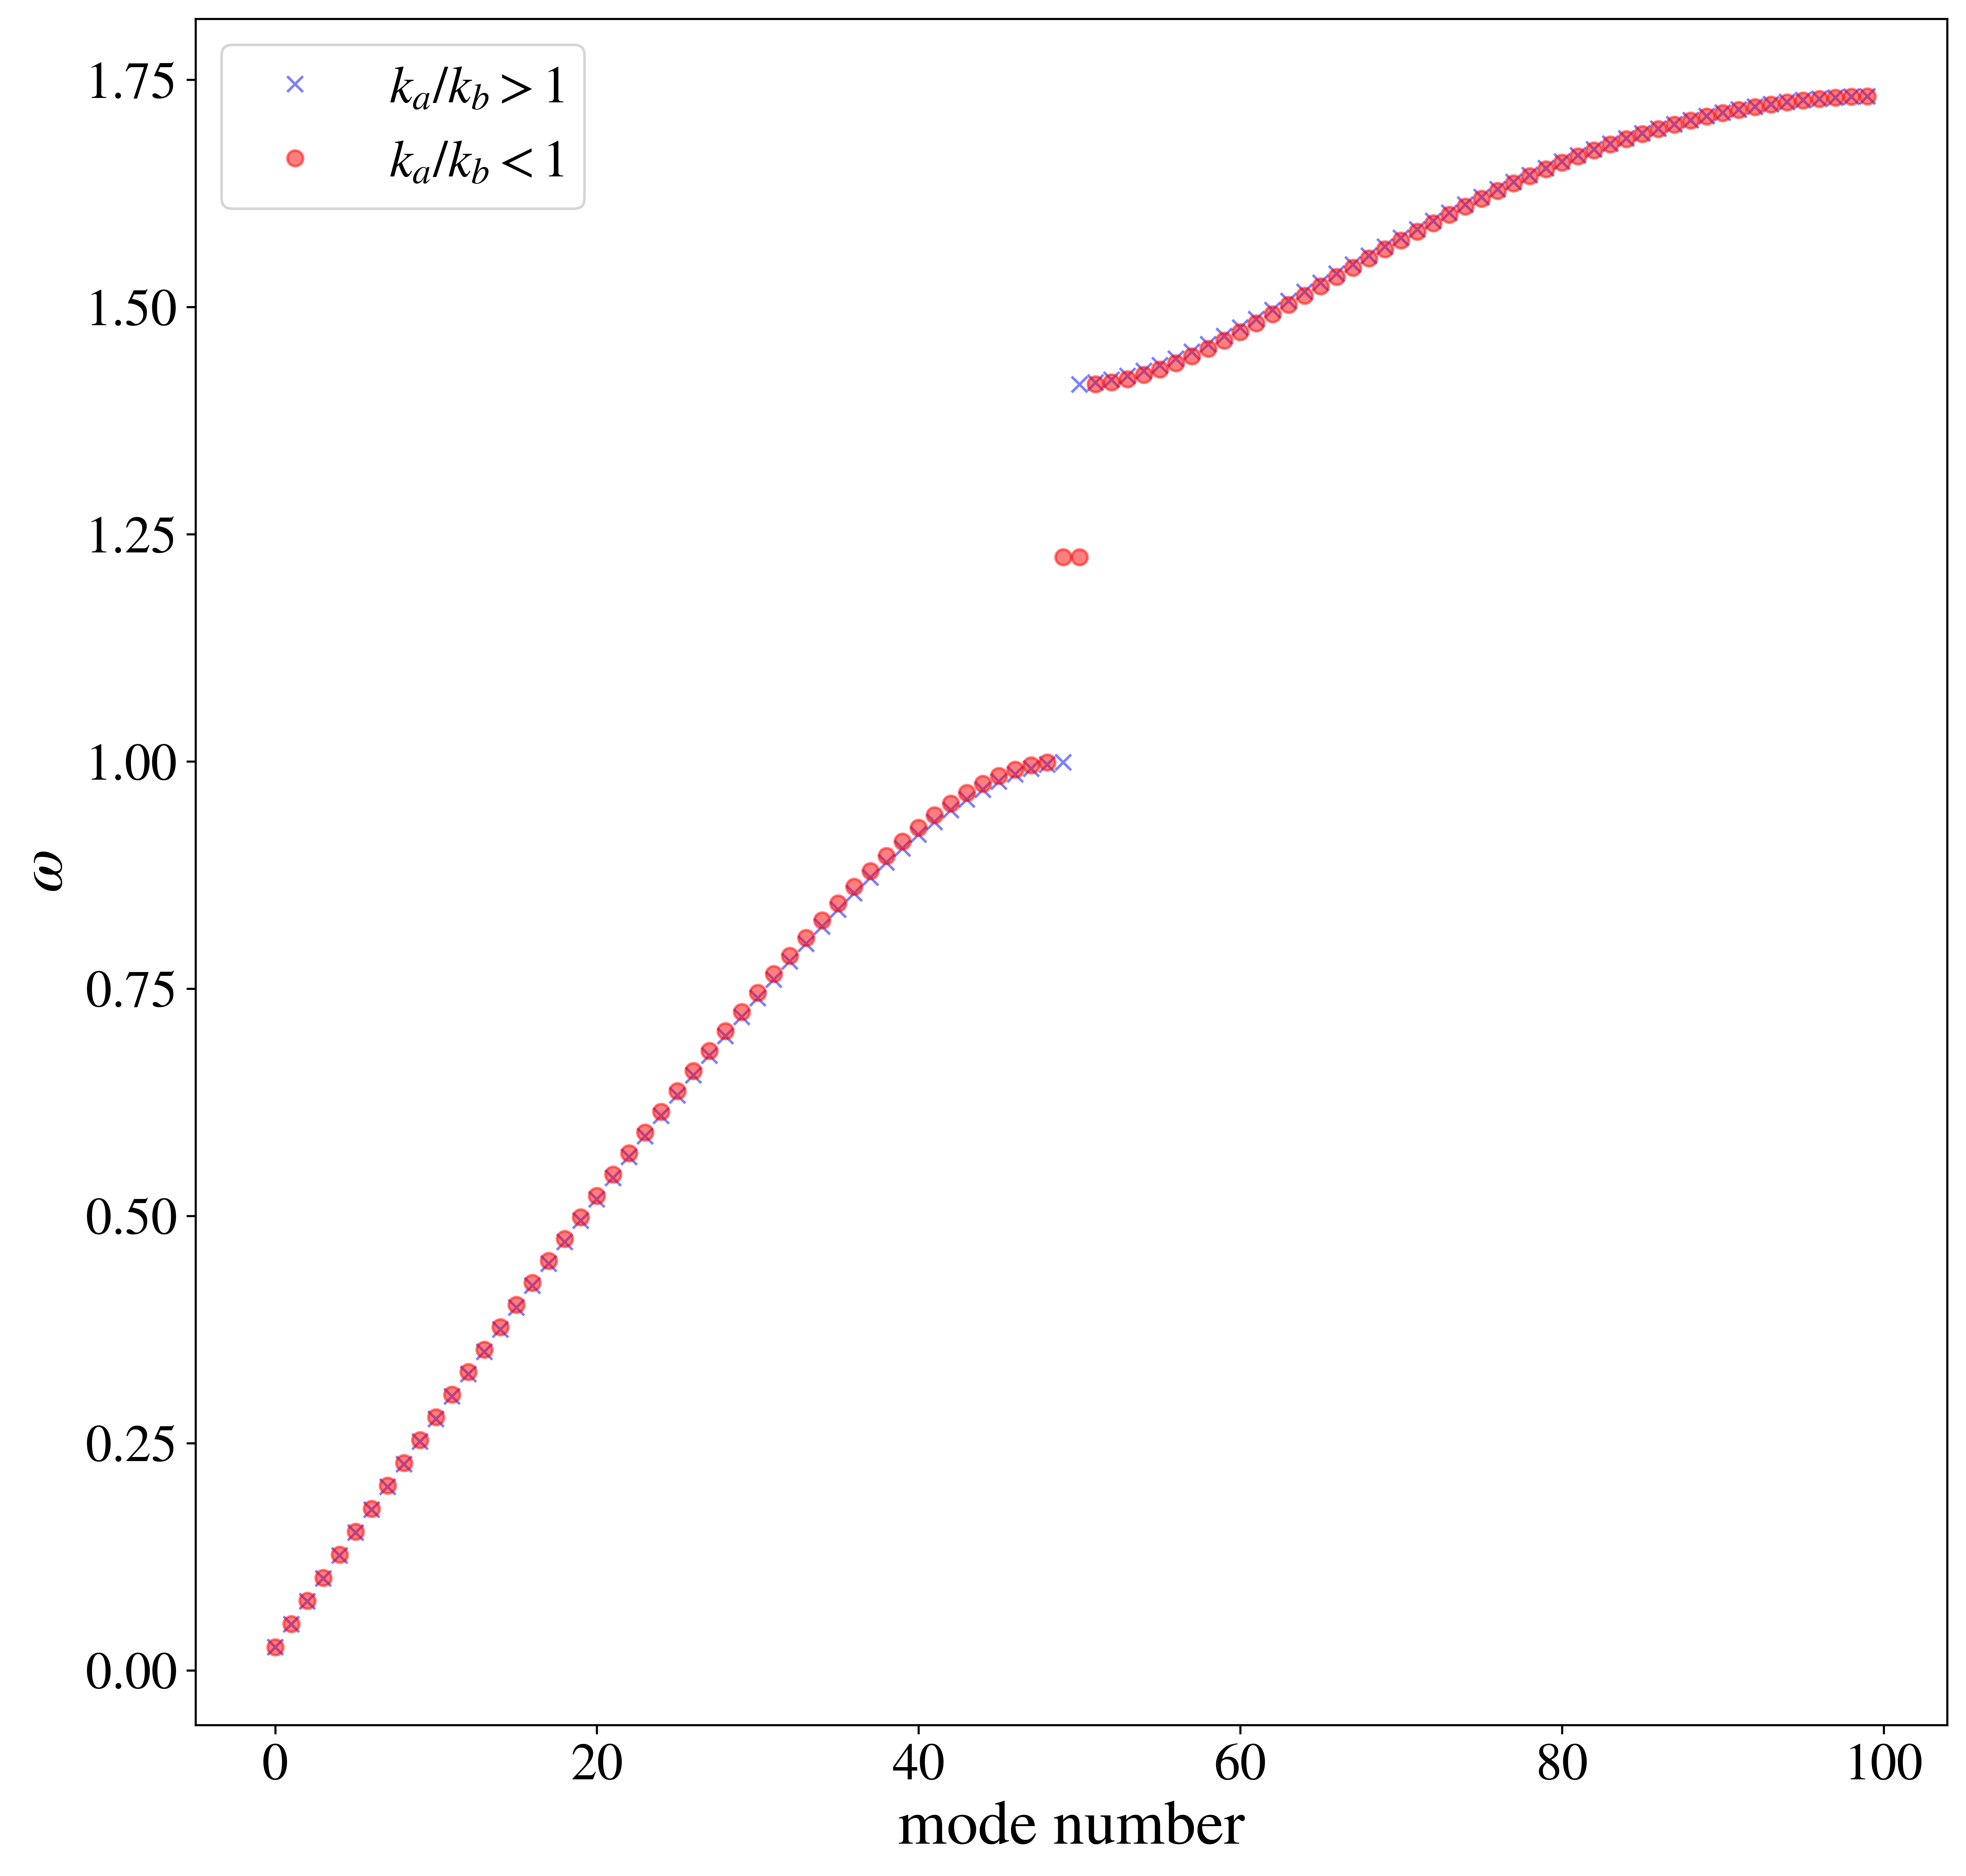
\includegraphics[width=\columnwidth]{ssh_fput_linear_modes.png}
    \caption{Dispersion relation for the acoustic SSH chain: }
    \label{fig:linear_modes}
\end{figure}

We use the SABA2C symplectic integrator described by\cite{2019Chaos..29b3132P}.
\section{\label{sec:methods}Linear Theory}
\begin{figure}
    \centering
    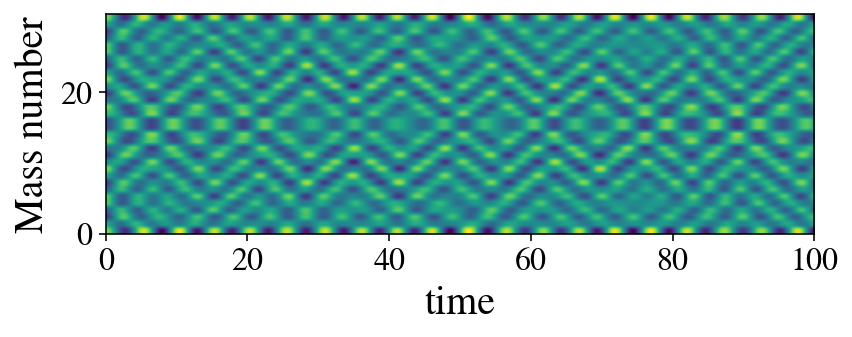
\includegraphics[width=\columnwidth]{ssh_linear_displacement_vs_time.png}
    \caption{Displacement as a function of mode number and time for a linear calculation with non-trivial topological phase $k_a > k_b$. Note the presence of non-propagating edge modes.}
    \label{fig:linear_displacement}
\end{figure}
\section{\label{sec:resuts}Results}
For a first experiment, we perform three runs all with the same initial conditions: $q_n = \sin(\pi n/L)$ with initial energy $E_0 = $
\appendix
Supplemental stuff goes here:
\begin{itemize}
    \item SABA2C error convergence
    \item time reversal test results table
\end{itemize}

\section{Nondimensionalization}
Take a mass, length, and time unit $M, L, T$.
Nondimensional quantities are marked with $\tilde{H}$.

\begin{equation}
    H = \frac{p^2}{2m} + k_i\left[\frac{(x_n - x_{n-1})^2}{2} + \alpha \frac{(x_n - x_{n-1})^3}{3}\right],
\end{equation}
where $k_i$ is $k_e$ if $n$ is even and $k_o$ if $n$ is odd.
If we choose $k_o T^2/M = 1$, then we get
\begin{equation}
    \tilde{H} = 
    \begin{cases}
    \frac{\tilde{p}^2}{2} + (\mathrm{To}+1)\left[\frac{(\tilde{x}_n - \tilde{x}_{n-1})^2}{2} + \alpha \frac{(\tilde{x}_n - \tilde{x}_{n-1})^3}{3}\right],  n\ \text{even}\\
    \frac{\tilde{p}^2}{2} + \left[\frac{(\tilde{x}_n - \tilde{x}_{n-1})^2}{2} + \alpha \frac{(\tilde{x}_n - \tilde{x}_{n-1})^3}{3}\right],  n\ \text{odd}\\
    \end{cases}
\end{equation}
with two control parameters $\alpha$ and $\mathrm{To} = (k_e - k_o)/k_o$. The former measures the strength of the nonlinear interaction, and the latter determines the topological protection: when $\mathrm{To} > 0$, the system is topologically protected.
\bibliography{topo}% Produces the bibliography via BibTeX.

\end{document}
%
% ****** End of file apssamp.tex ******
